\section{Rancangan Sistem Tiket}

\subsection{Komponen Sistem Tiket (tanpa Pengendalian Aliran)}

Komponen sistem tiket dapat dibagi menjadi beberapa bagian, yaitu layanan tiket, basis data relasional, dan kluster Redis. Komponen basis data relasional dapat dibagi menjadi tiga jenis, yaitu kluster PostgreSQL dengan replika baca, kluster CitusData, dan kluster YugabyteDB. Komponen ini yang akan menjadi sumber kebenaran utama dari sistem ini. Selain itu, kluster Redis digunakan untuk menyimpan data agregat ketersediaan berdasarkan area. Arsitektur ini diilustrasikan pada Gambar \ref{fig:ticket-nofc}.

\begin{figure}[H]
    \centering
    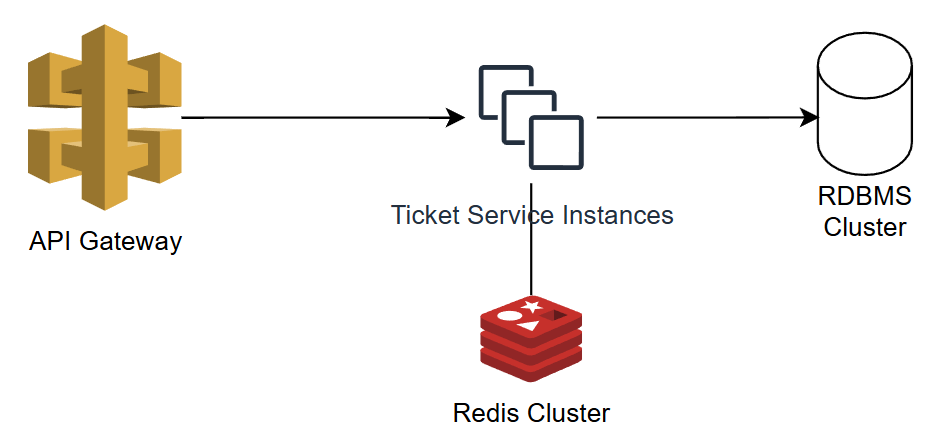
\includegraphics[width=0.8\textwidth]{resources/chapter-3/ticket-nofc.png}
    \caption{Diagram Arsitektur Sistem Tiket Tanpa Pengendalian Aliran}
    \label{fig:ticket-nofc}
\end{figure}

\pagebreak

\subsection{Komponen Sistem Tiket (dengan Pengendalian Aliran)}

Pada sistem tiket dengan pengendalian aliran, terdapat dua komponen baru yaitu RabbitMQ dan pemroses pesanan. RabbitMQ bertugas untuk menyimpan antrean permintaan pemesanan tiket dan pemroses pesanan bertugas untuk memproses pemesanan tiket. Selain itu, kluster Redis memiliki tanggung jawab tambahan untuk menyimpan data yang digunakan untuk menolak permintaan pesanan yang masuk lebih awal. Arsitektur ini diilustrasikan pada Gambar \ref{fig:ticket-fc}.

\begin{figure}[H]
    \centering
    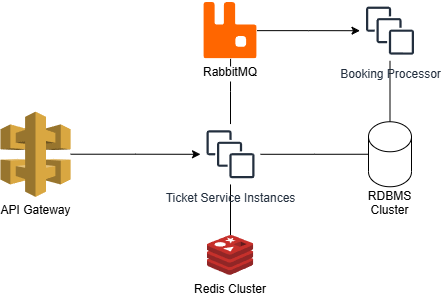
\includegraphics[width=0.8\textwidth]{resources/chapter-3/ticket-fc.png}
    \caption{Diagram Arsitektur Sistem Tiket dengan Pengendalian Aliran}
    \label{fig:ticket-fc}
\end{figure}

\subsection{Variasi Basis Data Relasional}

Untuk membandingkan pendekatan penskalaan yang berbeda, tiga arsitektur basis data diuji. Gambar \ref{fig:rdbms-variation} secara visual membedakan ketiganya: (1) kluster PostgreSQL standar dengan satu \textit{Primary} untuk tulis dan satu \textit{Replica} untuk baca; (2) kluster CitusData dengan satu Citus Coordinator yang mendistribusikan kueri ke beberapa Citus Worker; dan (3) kluster YugabyteDB dengan beberapa \textit{node} Master untuk metadata dan beberapa \textit{node} TServer untuk penyimpanan data.

\begin{figure}[H]
    \centering
    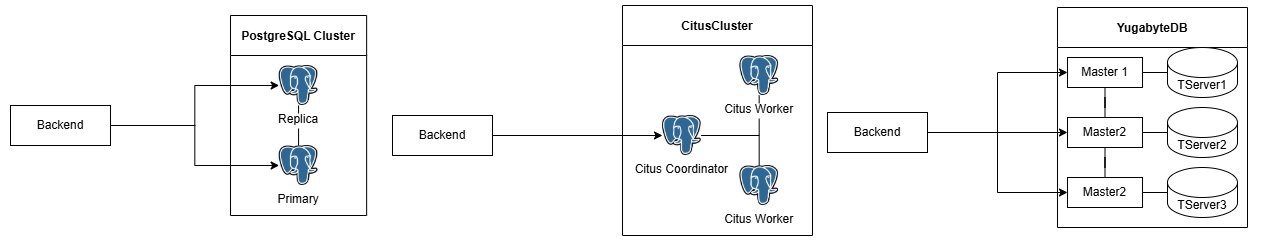
\includegraphics[width=1\textwidth]{resources/chapter-3/rdbms.png}
    \caption{Variasi Basis Data Relasional}
    \label{fig:rdbms-variation}
\end{figure}

Setiap varian memiliki alur eksekusi kueri dan model skalabilitas yang fundamental berbeda, yang berdampak langsung pada kinerja, terutama di bawah beban transaksi yang tinggi.

\subsubsection{Alur kueri pada Kluster PostgreSQL}

\begin{enumerate}
    \item \textbf{Alur kueri tulis:} Setiap permintaan yang mengubah data (misalnya, INSERT data pesanan baru atau UPDATE status kursi) harus diarahkan ke satu \textit{node} \textit{primary}. \textit{Pooler} PGCat akan mengidentifikasi jenis operasi ini dan secara eksklusif meneruskannya ke \textit{primary}. Setelah transaksi berhasil di-\textit{commit} pada \textit{primary}, perubahan tersebut kemudian direplikasi (pada kasus ini secara sinkron) ke \textit{node} \textit{replica}. Model ini menjamin konsistensi yang kuat tetapi menciptakan \textit{bottleneck} karena semua beban tulis terpusat pada satu mesin. Skalabilitas tulisnya terbatas pada penskalaan vertikal (meningkatkan sumber daya pada \textit{node} \textit{primary}).
    \item \textbf{Alur kueri baca:} Permintaan yang hanya membaca data (misalnya, SELECT untuk melihat ketersediaan kursi) dapat ditangani oleh \textit{primary} maupun \textit{replica}. Di sinilah peran PGCat menjadi krusial sebagai penyeimbang beban (\textit{load balancer}). PGCat mendistribusikan kueri baca ke kedua \textit{node}, sehingga beban baca dapat diskalakan secara horizontal dengan menambahkan lebih banyak \textit{replica}.
\end{enumerate}

\subsubsection{Alur kueri pada Kluster CitusData}

\begin{enumerate}
    \item \textbf{Alur Kueri Tulis:} Semua kueri dari aplikasi pertama-tama diterima oleh \textit{Citus Coordinator}. Untuk tabel yang telah didistribusikan seperti TicketSeats dan Orders, koordinator akan memeriksa kunci partisi (\textit{shard key}) dari data yang masuk (misalnya, ticket\_area\_id). Berdasarkan nilai kunci ini, koordinator menentukan secara tepat \textit{node Worker} mana yang menyimpan partisi data tersebut. Kueri kemudian diteruskan dan dieksekusi langsung pada \textit{worker} yang bersangkutan. Pendekatan ini memungkinkan operasi tulis untuk area tiket yang berbeda diproses secara paralel pada \textit{worker} yang berbeda, sehingga meningkatkan laju pemrosesan tulis secara keseluruhan dibandingkan dengan model \textit{Primary-Replica}.
    \item \textbf{Alur Kueri Baca:} Alur untuk kueri baca juga melalui koordinator. Jika kueri hanya menargetkan satu partisi, kueri akan diteruskan ke \textit{worker} yang relevan. Namun, untuk kueri agregat yang mencakup beberapa partisi, koordinator akan memecah kueri, mengirimkannya secara paralel ke beberapa \textit{worker}, lalu mengumpulkan dan menggabungkan hasilnya sebelum mengembalikannya ke aplikasi. Seluruh proses ini menciptakan \textit{overhead} pada koordinator yang bertanggung jawab atas perencanaan dan orkestrasi kueri terdistribusi.
\end{enumerate}

\subsubsection{Alur kueri pada Kluster YugabyteDB}

\begin{enumerate}
    \item \textbf{Alur Kueri Tulis:} Berbeda dengan arsitektur lain, YugabyteDB tidak memiliki satu \textit{node} penulis tunggal atau \textit{coordinator} sebagai \textit{bottleneck}. Aplikasi dapat terhubung ke \textit{node} \textit{TServer} mana pun untuk melakukan operasi tulis. Data secara otomatis dipecah menjadi unit-unit kecil yang disebut \textit{tablet}, yang didistribusikan ke seluruh \textit{TServer}. Setiap \textit{tablet} dikelola oleh sebuah grup konsensus Raft. Ketika sebuah \textit{TServer} menerima permintaan tulis, ia akan mengidentifikasi \textit{tablet leader} untuk data tersebut dan meneruskan permintaan jika diperlukan. \textit{Tablet leader} kemudian mengoordinasikan penulisan melalui protokol Raft, memastikan data direplikasi ke mayoritas \textit{node} sebelum mengonfirmasi keberhasilan transaksi. Alur ini memberikan skalabilitas tulis horizontal yang tinggi dan toleransi kegagalan, tetapi proses konsensus Raft untuk setiap penulisan menambah latensi jaringan.
    \item \textbf{Alur Kueri Baca:} Kueri baca yang membutuhkan konsistensi kuat (\textit{strong consistency}) akan diarahkan ke \textit{tablet leader}. Namun, YugabyteDB juga mendukung pembacaan dari \textit{follower} terdekat secara geografis untuk latensi yang lebih rendah dengan jaminan konsistensi yang sedikit lebih longgar (\textit{eventual consistency}).
\end{enumerate}

\subsubsection{Penggunaan \textit{Connection Pooler}}

\textit{Pooler} PGCat akan digunakan pada semua varian untuk mengelola koneksi basis data yang terbatas agar dapat digunakan ulang dan dipakai oleh klien yang lebih banyak. Pada konfigurasi kluster PostgreSQL, \textit{pooler} ini memiliki peran tambahan sebagai pembagi beban kueri baca antara \textit{primary} dan replika.

\subsection{Integrasi Layanan Pembayaran}

Sistem tiket terintegrasi dengan layanan pembayaran yang disimulasikan (\textit{mock service}). Rancangan layanan ini dibahas pada Lampiran \ref{apx:payment-service}.

\subsection{Alur Sistem Tiket}

\subsubsection{Alur Fitur Acara}

Alur untuk berbagai fitur terkait acara diilustrasikan pada Gambar \ref{fig:flow-event}. Diagram ini menunjukkan tiga alur permintaan opsional (opt) dari User ke Ticket Backend:

\begin{enumerate}
    \item Untuk detail acara, sistem langsung melakukan kueri ke Database.
    \item Untuk ketersediaan area secara agregat, sistem mengambil data yang sudah diolah dari Redis, sehingga mengurangi beban pada basis data utama.
    \item Untuk ketersediaan kursi, diagram menunjukkan blok alternatif (alt). Sistem pertama-tama memeriksa cache di memori internal. Jika data ditemukan, data akan langsung dikembalikan (\textit{cache hit}). Jika tidak (\textit{cache miss}), sistem akan melakukan kueri ke Database, menyimpan hasilnya di-\textit{cache} untuk permintaan berikutnya, lalu mengembalikannya ke pengguna.
\end{enumerate}

\begin{figure}[H]
    \centering
    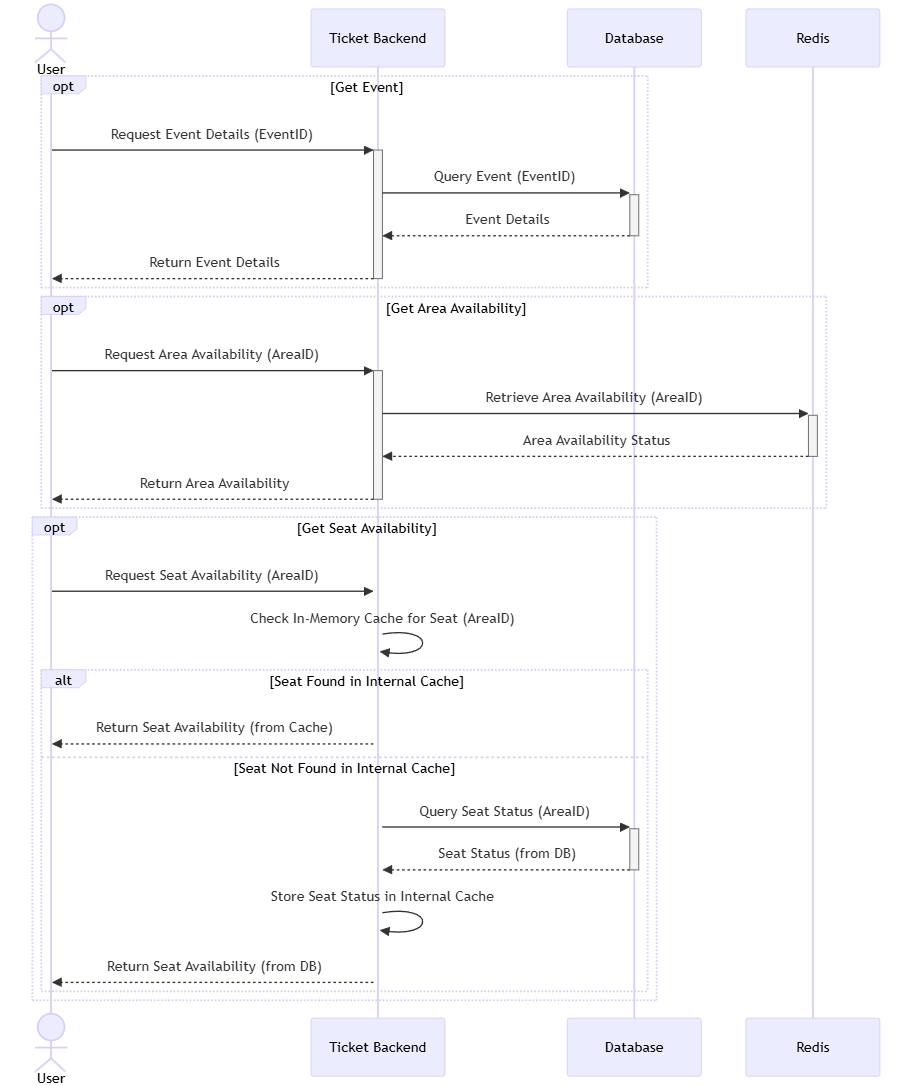
\includegraphics[width=1\textwidth]{resources/chapter-3/event-flow.png}
    \caption{Diagram Alur Fitur acara}
    \label{fig:flow-event}
\end{figure}

\subsubsection{Alur Fitur Pemesanan Tiket (tanpa pengendalian aliran)}

Proses pemesanan tiket tanpa pengendalian aliran, yang diilustrasikan pada Gambar \ref{fig:flow-book-flow}, dirancang untuk menjaga integritas data. Alurnya adalah sebagai berikut: setelah menerima permintaan, sistem pertama-tama melakukan pengecekan idempotensi di Redis untuk mencegah pemrosesan duplikat. Jika ini adalah permintaan baru, Ticket Backend akan memulai transaksi (Begin Transaction) dengan Database. Langkah krusialnya adalah melakukan kueri penguncian baris (Lock seat rows) untuk memastikan kursi yang dipilih tidak dapat dipesan oleh transaksi lain secara bersamaan. Jika kursi tidak tersedia atau gagal dikunci, transaksi akan dibatalkan (Rollback). Jika berhasil, sistem akan membuat tagihan di Payment Backend, menyimpan informasi pesanan, dan akhirnya melakukan Commit Transaction untuk menyelesaikan pemesanan.

\begin{figure}[H]
    \centering
    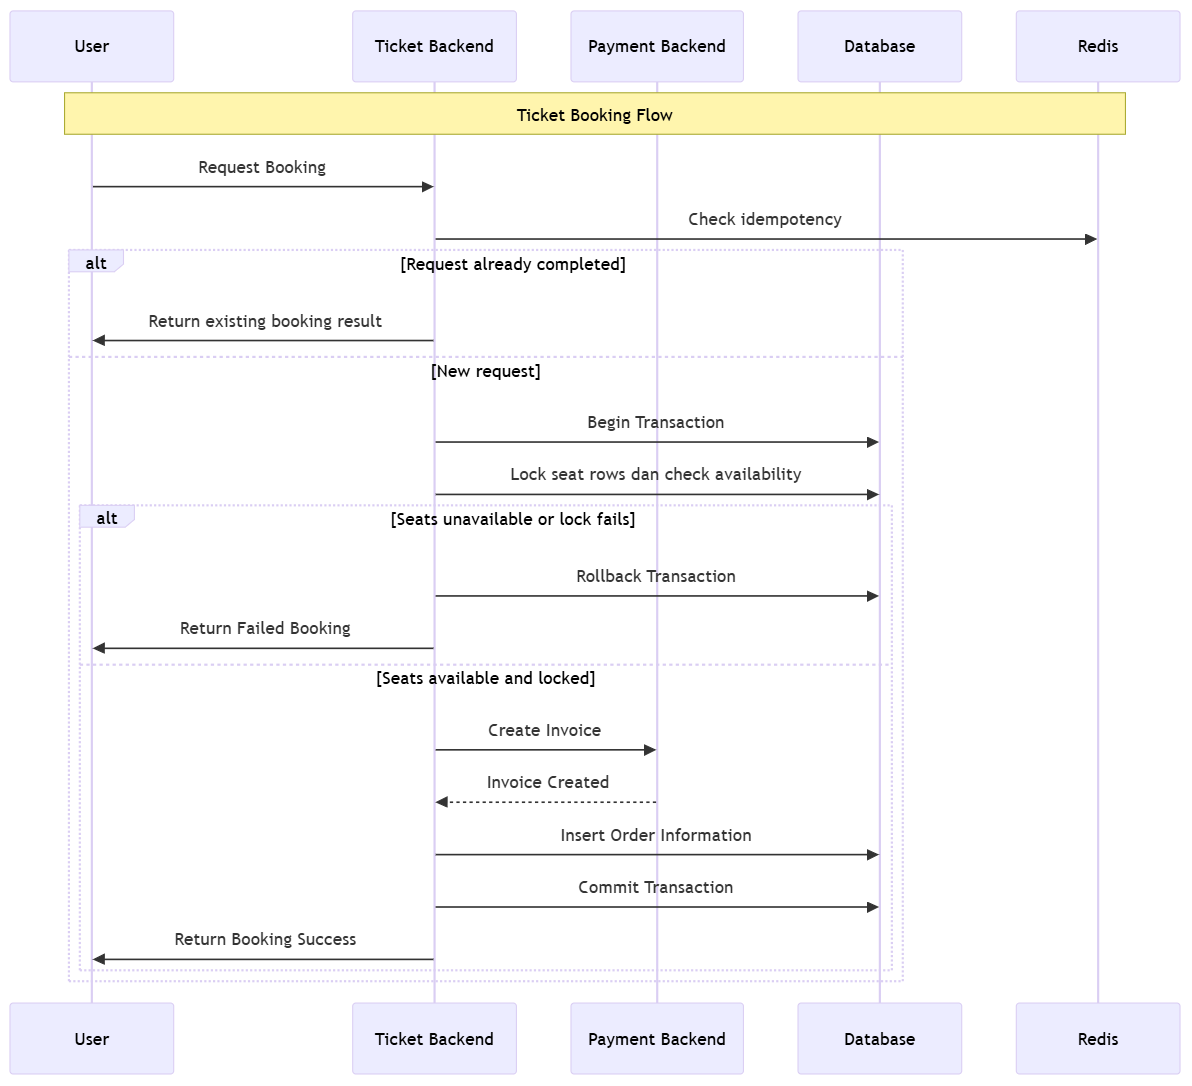
\includegraphics[width=1\textwidth]{resources/chapter-3/book-flow.png}
    \caption{Diagram Alur Fitur Pemesanan Tiket (tanpa pengendalian aliran)}
    \label{fig:flow-book-flow}
\end{figure}

Alur pembayaran dan konfirmasi tiket, seperti yang ditunjukkan pada Gambar \ref{fig:flow-order-payment-flow}, melibatkan dua proses yang berjalan paralel. Pertama, User berinteraksi langsung dengan Payment Backend untuk membayar tagihan (Pay Invoice). Kedua, dan yang lebih penting, diagram ini menunjukkan proses notifikasi asinkron dalam blok par. Payment Backend secara independen mengirimkan webhook (Notify Payment Status Update) ke Ticket Backend. Bergantung pada status pembayaran, Ticket Backend kemudian akan memperbarui status pesanan, menerbitkan tiket (Insert Published Ticket), dan mengoreksi data agregat ketersediaan di Redis. Pengguna kemudian dapat secara terpisah memeriksa status pesanan mereka, yang sudah diperbarui oleh proses di latar belakang ini.

\begin{figure}[H]
    \centering
    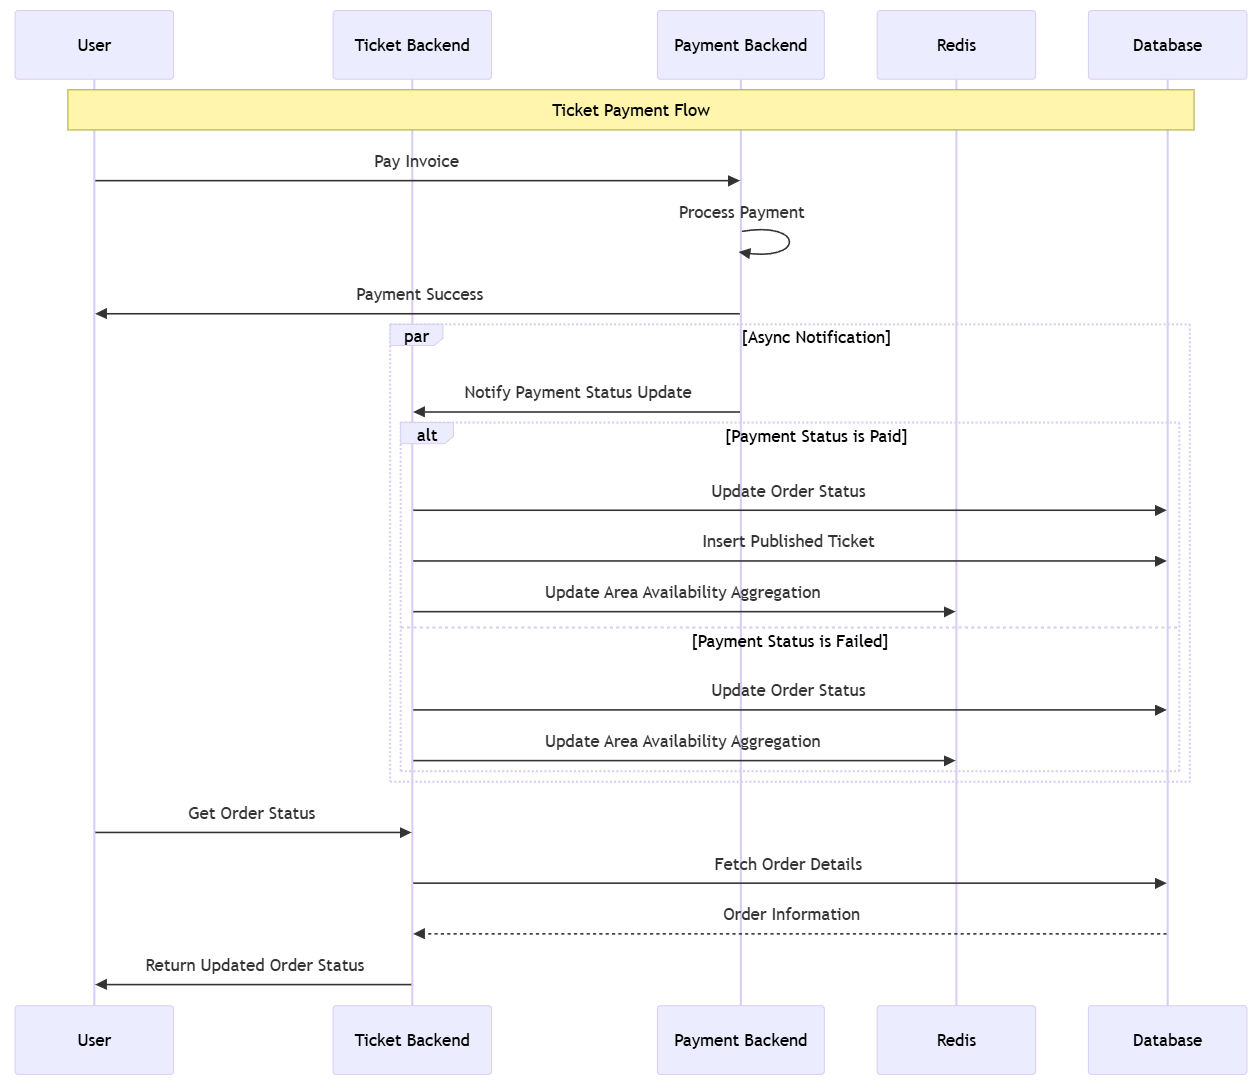
\includegraphics[width=1\textwidth]{resources/chapter-3/order-payment.png}
    \caption{Diagram Alur Fitur Pembayaran Tiket (tanpa pengendalian aliran)}
    \label{fig:flow-order-payment-flow}
\end{figure}

\subsubsection{Alur Fitur Pemesanan Tiket (dengan pengendalian aliran)}

Alur pemesanan tiket dengan pengendalian aliran, yang dirinci pada Gambar \ref{fig:flow-book-fc}, memperkenalkan antrean untuk mengatur beban ke basis data. Prosesnya sebagai berikut: setelah cek idempotensi, sistem melakukan pengecekan kedua di Redis untuk menolak permintaan lebih awal jika kursi yang sama sedang dalam proses pemesanan lain. Jika lolos, Ticket Backend tidak langsung ke basis data, melainkan mempublikasikan permintaan ke antrean di RabbitMQ dan menunggu pesan balasan. Di sisi lain, sebuah Ticket Worker mengambil pesan dari antrean tersebut (bagian "Worker Processing"). Worker inilah yang bertanggung jawab menjalankan transaksi basis data yang intensif (mengunci baris, membuat tagihan, dan commit). Setelah selesai, worker mengirimkan hasilnya kembali melalui antrean balasan, yang kemudian diterima oleh Ticket Backend dan diteruskan kepada User. Alur ini mengubah pemrosesan yang tadinya sinkron menjadi asinkron untuk menjaga stabilitas.

\begin{figure}[H]
    \centering
    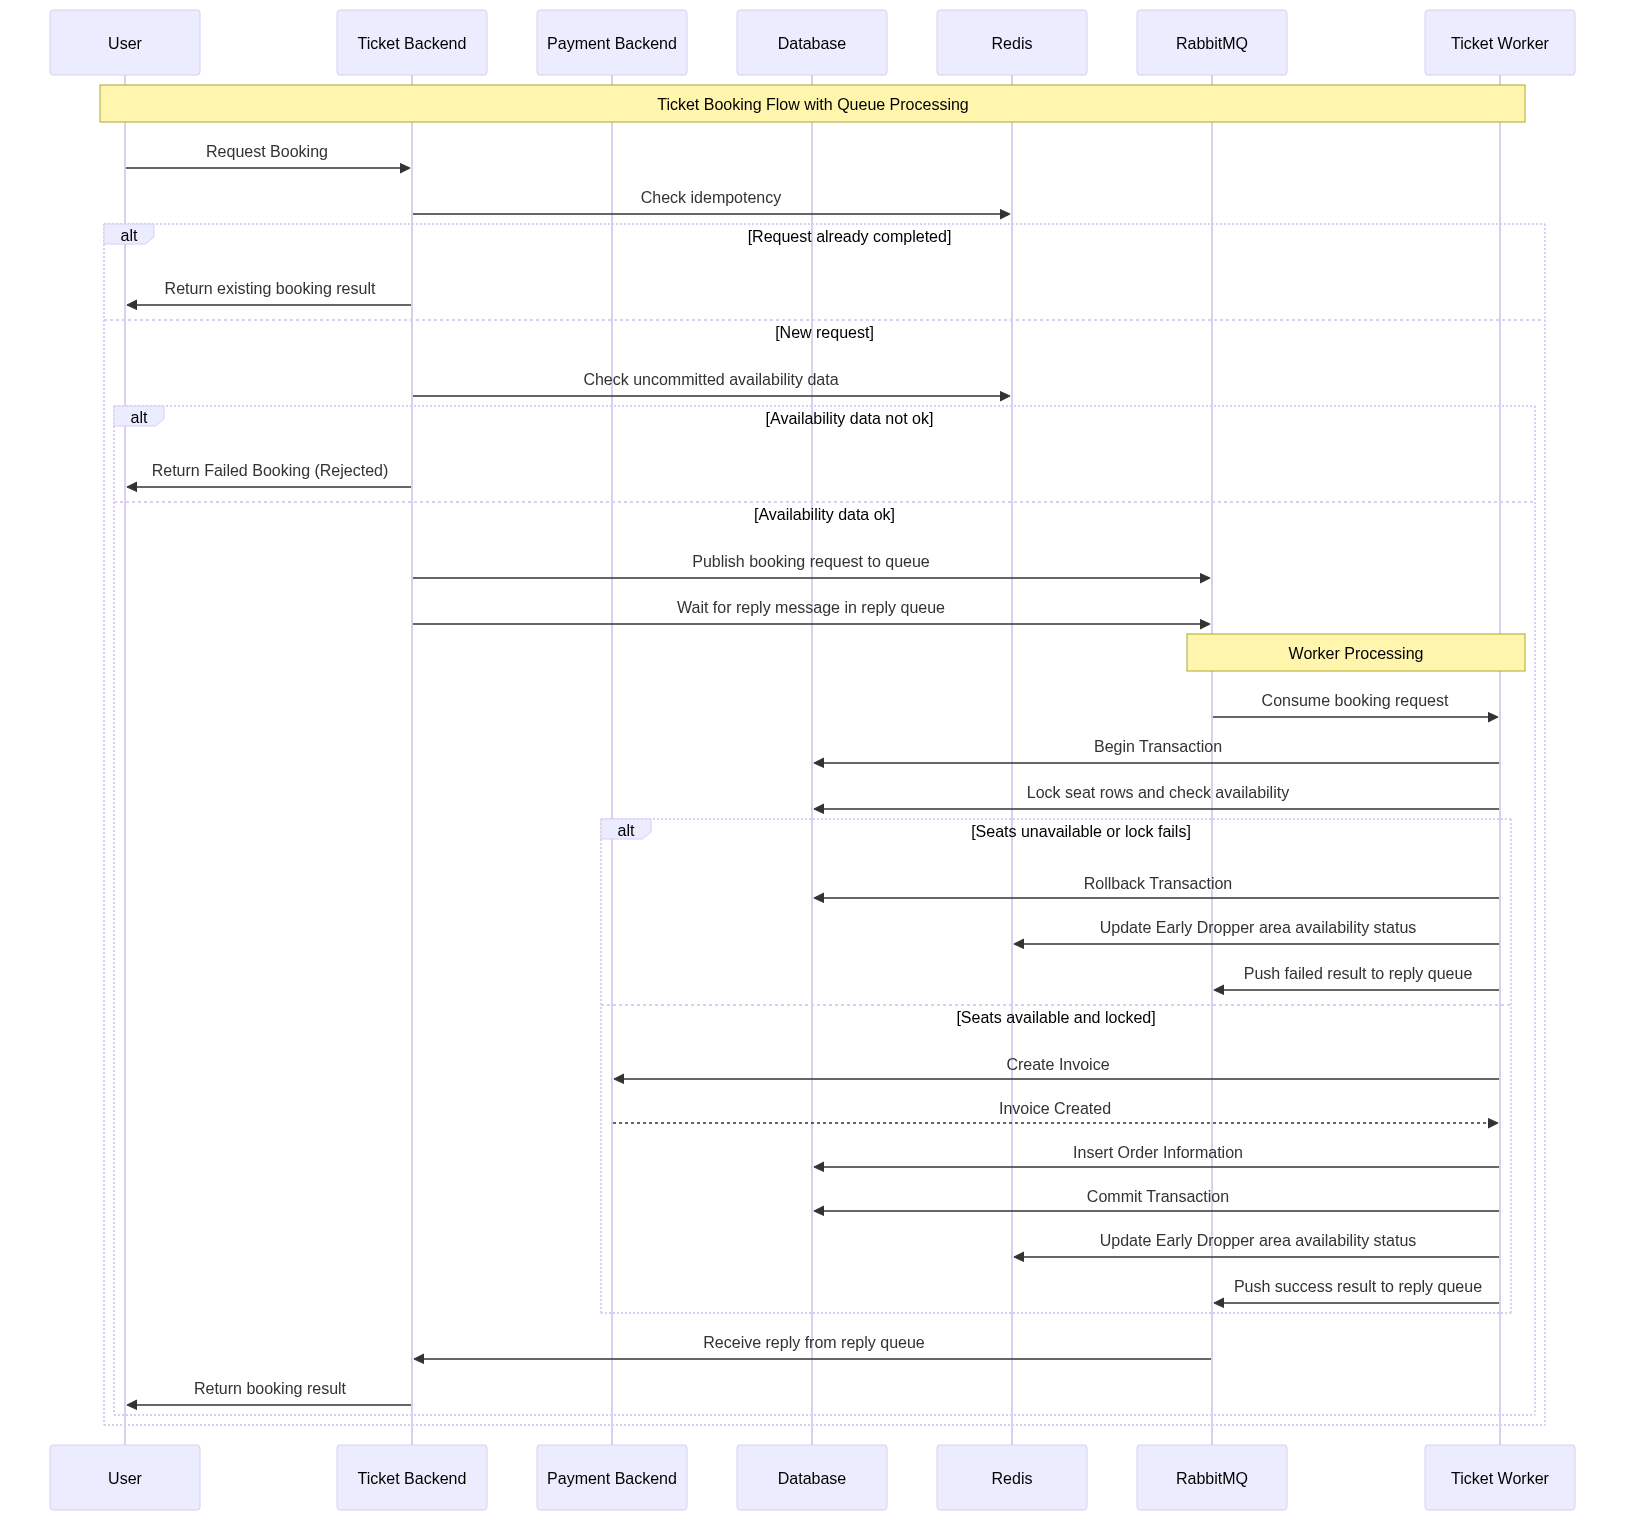
\includegraphics[width=1\textwidth]{resources/chapter-3/book-async.png}
    \caption{Diagram Alur Fitur Pemesanan Tiket (dengan pengendalian aliran)}
    \label{fig:flow-book-fc}
\end{figure}

Ketika pengguna berhasil memesan, pengguna akan melakukan pembayaran kepada gerbang pembayaran. Setelah pembayaran selesai, pengguna memeriksa status pesanan yang telah dibuat. Tidak ada perbedaan signifikan selain pembaruan data pada Redis untuk sinkronisasi data yang menjadi basis untuk menolak permintaan pesanan lebih awal. Alur fitur ini diilustrasikan pada Gambar \ref{fig:flow-order-payment-fc}.

\begin{figure}[H]
    \centering
    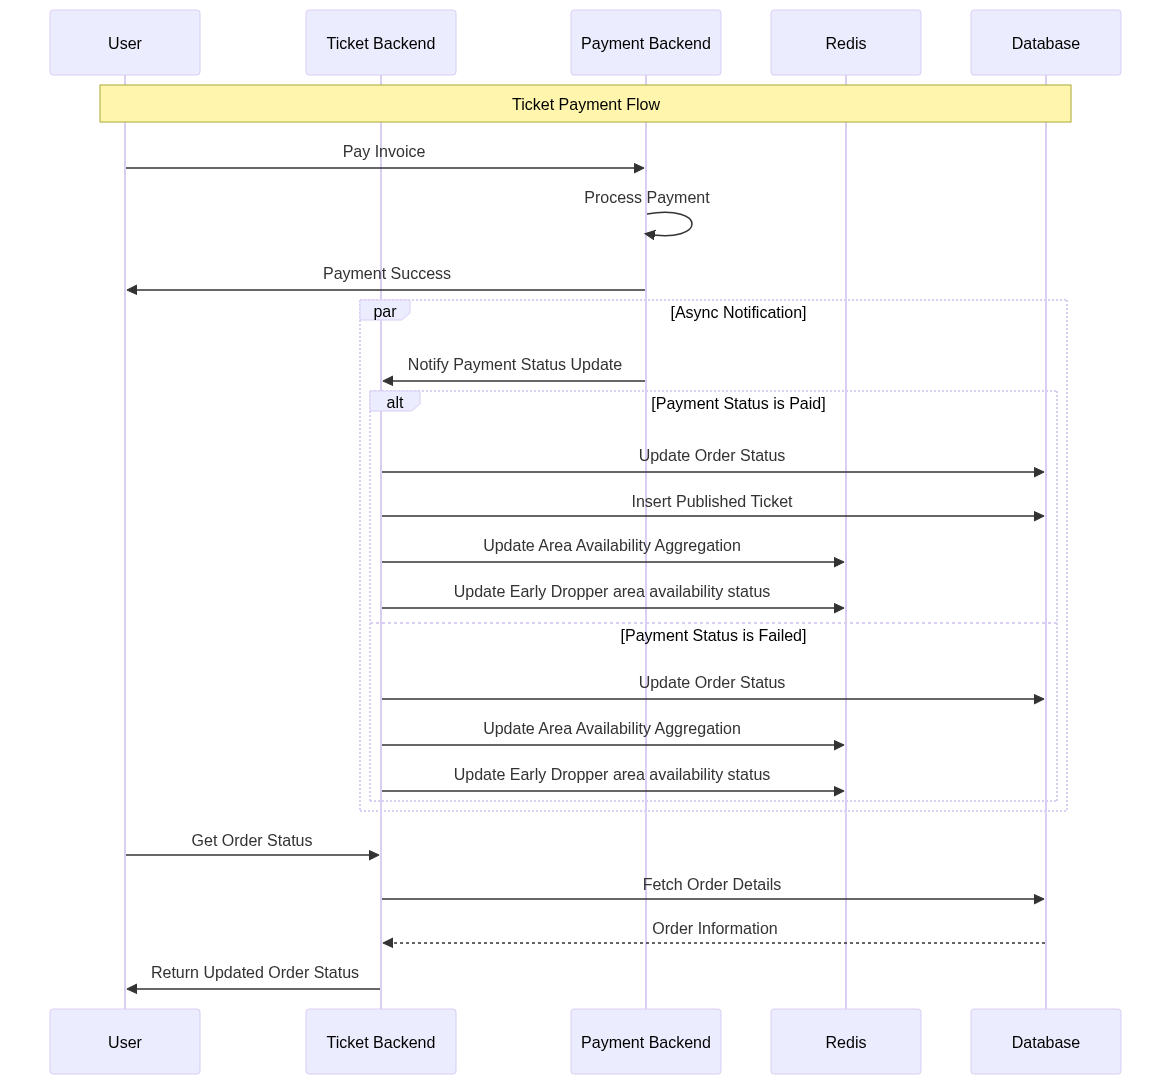
\includegraphics[width=1\textwidth]{resources/chapter-3/order-payment-fc.png}
    \caption{Diagram Alur Fitur Pembayaran Tiket (dengan pengendalian aliran)}
    \label{fig:flow-order-payment-fc}
\end{figure}

\subsubsection{Alur Fitur Pembacaan Pesanan}

Terdapat dua operasi tambahan yang berkaitan dengan pembacaan pesanan, yaitu membaca detail pesanan dan membaca tiket yang sudah diterbitkan. Alur fitur ini diilustrasikan pada Gambar \ref{fig:flow-order-flow}. Diagram tersebut memvisualisasikan bagaimana Pengguna dapat meminta status pesanan atau tiket yang telah terbit. Dalam kedua skenario opsional ini, Ticket Backend menerima permintaan, mengambil informasi yang sesuai dari Database, dan mengembalikannya kepada Pengguna. Proses ini memastikan bahwa data yang ditampilkan kepada pengguna selalu yang paling terbaru.

\begin{figure}[H]
    \centering
    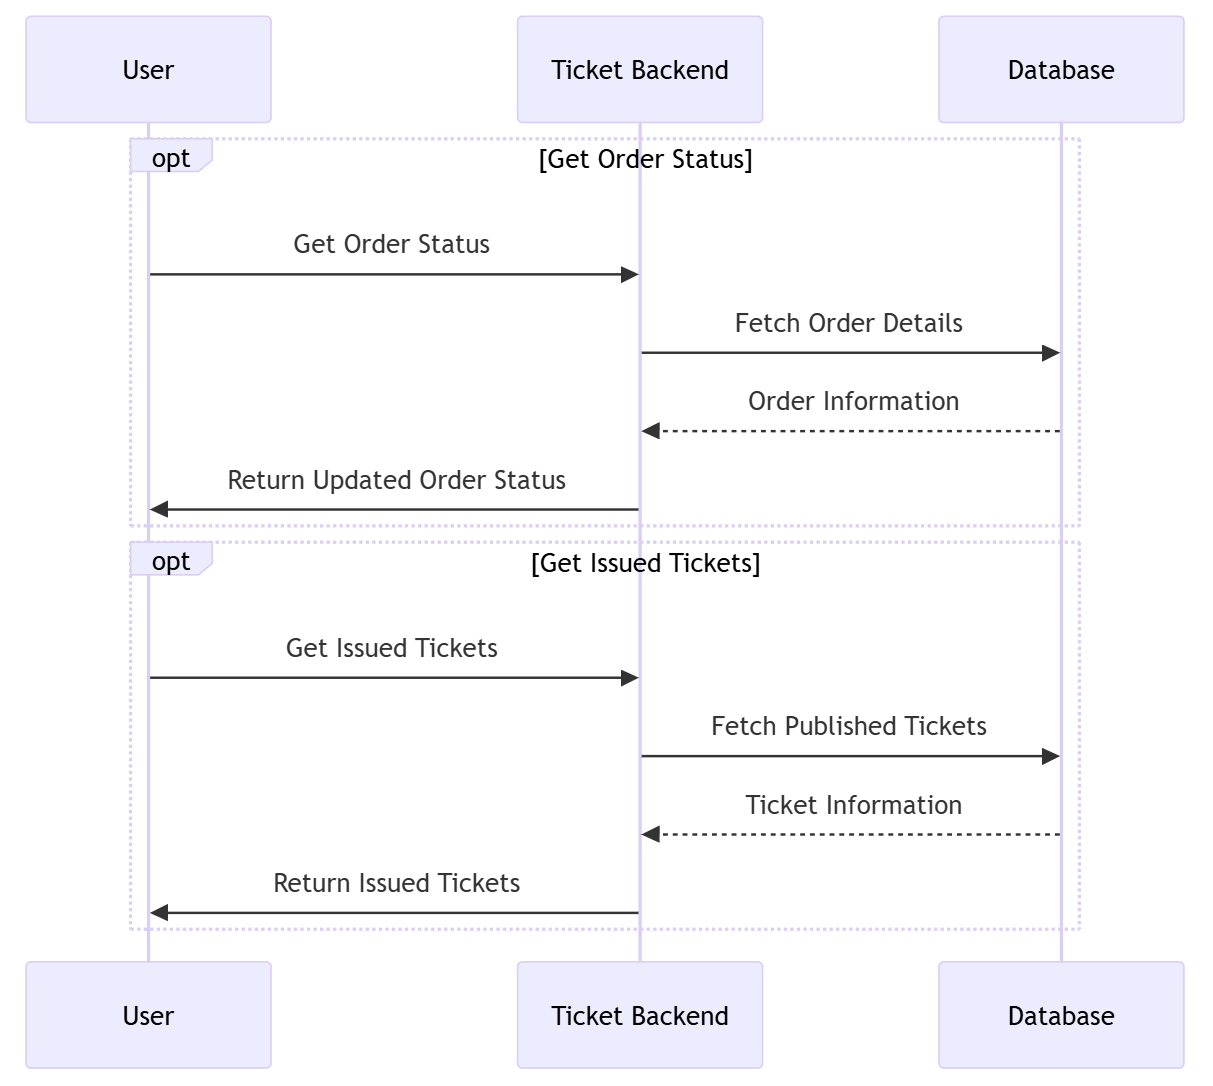
\includegraphics[width=1\textwidth]{resources/chapter-3/order-flow.png}
    \caption{Diagram Alur Fitur Pembacaan Pesanan}
    \label{fig:flow-order-flow}
\end{figure}